% !TeX root = ../../../main.tex
\subsection{Introduction}

%%%%%%%%%%%%%%%%%%%%%%%%%%%%%%%%%%%%%%%%%%%%%%%%%
%%%%%%%%%%%%%%% Revised Intro %%%%%%%%%%%%%%%%%%%%%%
%%%%%%%%%%%%%%%%%%%%%%%%%%%%%%%%%%%%%%%%%%%%%%%%
Healthcare disparities persist globally, with preventable deaths from conditions like sepsis disproportionately affecting underserved populations who often present to under-resourced facilities with limited access to specialized expertise.
In these settings, much of the critical diagnostic and prognostic information exists only in unstructured clinical narratives—case reports, discharge summaries, and progress notes—as comprehensive structured data infrastructure may be unavailable~\cite{anzalone2025lower,seinen2025using}.
While machine learning approaches have shown promise on structured data, with recent work demonstrating that incorporating text alongside structured inputs significantly improves predictive performance~\citep{kline2022multimodal}, large language models struggle with clinical risk estimation, especially in patient-facing scenarios~\citep{wongposition}.
This gap highlights the need for automated risk forecasting from textual clinical records that could democratize access to expert-level clinical reasoning, particularly in resource-constrained environments where timely specialist consultation is not available.
The challenge of LLM risk estimation motivates a structured treatment of risk forecasting and survival modeling from unstructured narrative sources.

Among textual sources, retrospective case reports serve as a rich training ground for developing temporally-aware AI systems that can eventually be deployed on real-time clinical notes.
Case reports provide holistic accounts of clinical trajectories with explicit temporal reasoning—exactly the type of structured thinking needed for real-time clinical decision support.
However, their narrative structure interleaves temporally unordered information, making them difficult to apply in forecasting tasks.
Without identifying the time of occurrence for each event, models are prone to causal leakage—using information not available at the time of prediction.
Solving this temporal reasoning challenge in case reports establishes the foundation for deployment in live clinical environments where such capabilities could improve patient outcomes.

% \begin{figure*}[!tbp] % 'r' for right, 'l' for left
%     \centering
%     \includegraphics[width=.95\linewidth]{AAAI_2026/Figures/annotation_ex.png} % Adjust width
%     \caption{Example case report (left) with timeline representations (middle) and text-ordered, (event, time) tuples (right).}
%     \label{fig:annotation_ex}
%     % \vspace{-5mm}
% \end{figure*}


% !TeX root = ../../../main.tex
\begin{figure}[htbp]
\begin{ChSevenFloatBody}
    \centering
    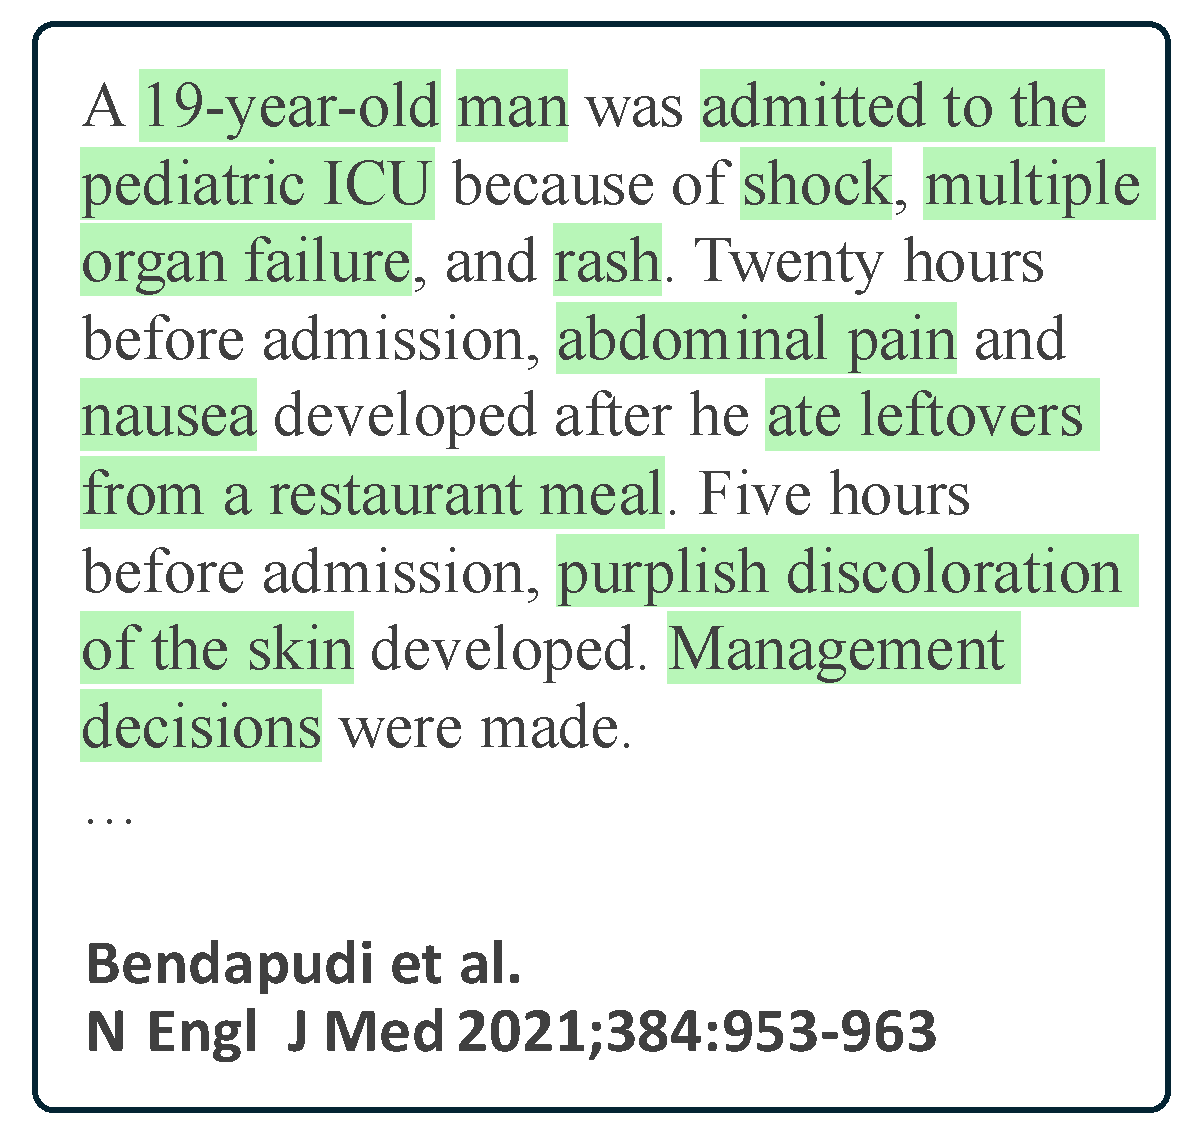
\includegraphics[page=1,width=.33\linewidth]{Chapters/chapter-07/images/Figures/annotation_ex_updated.pdf}%
    \includegraphics[page=2,width=.33\linewidth]{Chapters/chapter-07/images/Figures/annotation_ex_updated.pdf}%
    \includegraphics[page=3,width=.33\linewidth]{Chapters/chapter-07/images/Figures/annotation_ex_updated.pdf}%
    
    

\end{ChSevenFloatBody}
\caption{Example case report (left) with timeline representations (middle) and text-ordered, (event, time) tuples (right).}\ChSevenFloatLabel{ch07:fig:annotation_ex}
\end{figure}


One might ask whether large pretrained language models can already perform forecasting from clinical narratives, given their exposure to biomedical texts~\citep{peng2020empirical,weber2024redpajama}.
However, these models have architectural limitations for temporal reasoning tasks.
Encoder-based models apply random masking that rarely yields temporally coherent representations, while decoder-style models mask text in linear sequence, modeling events in text order rather than time order. 
Our experiments make these limitations explicit.
For instance, on the timeline in Figure \ref{ch07:fig:annotation_ex}, the chance of recovering a valid time-ordered mask is below $0.002\%$, and decoder models show low temporal concordance (e.g., $c=0.23$).
Without a task-specific restructuring, such factors lead to suboptimal forecasting performance.
% Our experiments demonstrate these limitations quantitatively---for example, using the timeline in Figure~\ref{ch07:fig:annotation_ex}, the probability of recovering a valid time-ordered mask is $<0.002\%$, and decoder models achieve low temporal concordance (e.g., $c=0.23$), leading to suboptimal forecasting accuracy without task-specific restructuring.

To address these temporal reasoning challenges, we develop a forecasting framework that
%similar to \citet{noroozizadeh2025reconstructing}
transforms free-text narratives into textual time series---sequences of (event, time) tuples---and makes explicit the temporal structure of patient trajectories.
Building on recent annotation work~\citep{wang2025large,noroozizadeh2025pmoa}, we propose a hybrid pipeline combining rule-based heuristics and LLM-assisted extraction to recover temporally localized clinical findings, validated on real clinical notes with expert verification.

Our work builds on extensive research in clinical NLP and temporal reasoning~\citep{kohane1987temporal,leeuwenberg2020towards,cheng2023typed}, but shifts the emphasis from extraction to downstream clinical forecasting.
While prior efforts have focused on entity recognition and temporal relation extraction \citep{zhou2007temporal,ch07:uzuner20112010,sun2013evaluating}, few have systematically assessed how such representations influence downstream tasks such as risk prediction and survival modeling.
We bridge this gap by formalizing textual time series representations and evaluating their effectiveness for temporally grounded clinical prediction.

We empirically assess this framework across multiple tasks and modeling strategies, benchmarking encoder and decoder models—both fine-tuned and prompted versions—on three forecasting tasks: event prediction, survival analysis, and temporal ordering of future clinical events.
Our results show no single model dominates across all tasks, highlighting the importance of aligning model architecture with forecasting objectives.
We further examine how input ordering (time vs. narrative) impacts generalization and analyze the sensitivity of models to missing historical context through systematic masking experiments.

% \textbf{Contributions.} 
{\raggedright
In summary, this paper makes the following contributions:

(i) \textbf{Annotation and Extraction Pipeline:} Building on prior methods for extracting information from the PubMed Open Access corpus \cite{ch07:noroozizadeh2025reconstructing}, this work introduces a pipeline that transforms case reports into textual time series via regular expression filtering and LLM-assisted extraction, yielding temporally anchored (event, time) tuples while minimizing causal leakage by restricting input to past events;
\mbox{(ii) \textbf{Comprehensive Model Comparison:}} 
    We conduct a comprehensive evaluation of encoder- and instruction-tuned decoder-based models—using both fine-tuned MLP heads and prompting—across event prediction, temporal ordering, and survival analysis tasks.
Results show no single model excels universally, underscoring the need to align model choice with the specific forecasting objective;
\mbox{(iii) \textbf{Temporal- versus Text- Ordering:}}
    We investigate the impact of annotation order by comparing training on time-ordered versus text-ordered data.
Results show that preserving the narrative's natural order can improve generalization to external datasets, while time-based ordering can enhance ranking performance;
    %in certain settings.
\mbox{(iv) \textbf{Sensitivity Analysis of Temporal Masking:}}
    We conduct systematic dropout experiments by randomly masking parts of the clinical history to assess their impact on forecasting and event ordering.
While higher masking levels reduce classification performance (F1), the concordance index remains largely stable, highlighting differing sensitivities of binary prediction and ranking tasks to historical context in textual time series;
(v) \textbf{Methodological Framework for Temporal Clinical Forecasting:} Our approach demonstrates how narrative clinical texts can be systematically converted into structured temporal representations for forecasting tasks, providing a replicable methodology that could be adapted to other clinical and non-clinical text sources. 


%%%%%%%%%%%%%%%%%%%%%%%%%%%%%%%%%%%%%%%%%%%%%
%%%%%%%%%%%%%%% Related Work %%%%%%%%%%%%%%%%
%%%%%%%%%%%%%%%%%%%%%%%%%%%%%%%%%%%%%%%%%%%%%
\par}
